% Created by tikzDevice version 0.12.6 on 2026-05-14 19:53:57
% !TEX encoding = UTF-8 Unicode
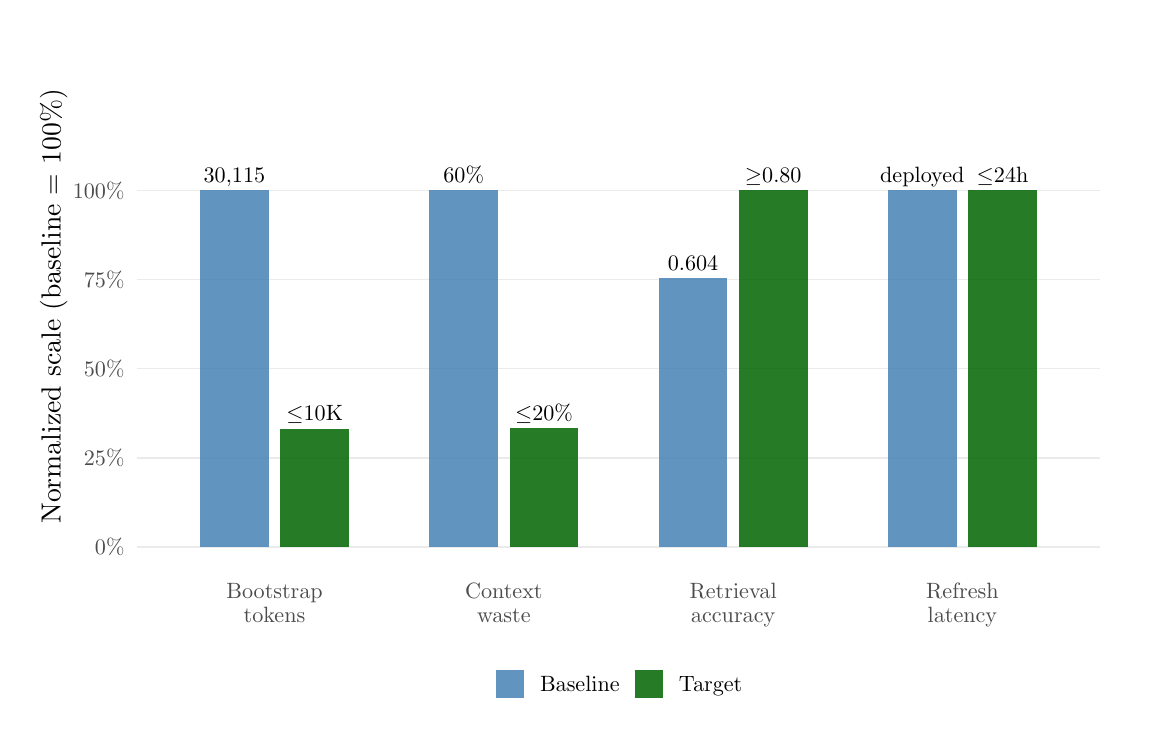
\begin{tikzpicture}[x=1pt,y=1pt]
\definecolor{fillColor}{RGB}{255,255,255}
\path[use as bounding box,fill=fillColor,fill opacity=0.00] (0,0) rectangle (397.48,252.94);
\begin{scope}
\path[clip] (  0.00,  0.00) rectangle (397.48,252.94);
\definecolor{fillColor}{RGB}{255,255,255}

\path[fill=fillColor] (  0.00,  0.00) rectangle (397.48,252.94);
\end{scope}
\begin{scope}
\path[clip] ( 39.49, 56.59) rectangle (387.48,247.95);
\definecolor{drawColor}{gray}{0.92}

\path[draw=drawColor,line width= 0.5pt,line join=round] ( 39.49, 65.28) --
	(387.48, 65.28);

\path[draw=drawColor,line width= 0.5pt,line join=round] ( 39.49, 97.50) --
	(387.48, 97.50);

\path[draw=drawColor,line width= 0.5pt,line join=round] ( 39.49,129.71) --
	(387.48,129.71);

\path[draw=drawColor,line width= 0.5pt,line join=round] ( 39.49,161.93) --
	(387.48,161.93);

\path[draw=drawColor,line width= 0.5pt,line join=round] ( 39.49,194.15) --
	(387.48,194.15);
\definecolor{fillColor}{RGB}{70,130,180}

\path[fill=fillColor,fill opacity=0.85] ( 62.28, 65.28) rectangle ( 87.14,194.15);

\path[fill=fillColor,fill opacity=0.85] (145.13, 65.28) rectangle (169.99,194.15);

\path[fill=fillColor,fill opacity=0.85] (227.99, 65.28) rectangle (252.85,162.57);

\path[fill=fillColor,fill opacity=0.85] (310.84, 65.28) rectangle (335.70,194.15);
\definecolor{fillColor}{RGB}{0,100,0}

\path[fill=fillColor,fill opacity=0.85] ( 91.28, 65.28) rectangle (116.13,108.07);

\path[fill=fillColor,fill opacity=0.85] (174.13, 65.28) rectangle (198.99,108.24);

\path[fill=fillColor,fill opacity=0.85] (256.99, 65.28) rectangle (281.84,194.15);

\path[fill=fillColor,fill opacity=0.85] (339.84, 65.28) rectangle (364.70,194.15);
\definecolor{drawColor}{RGB}{0,0,0}

\node[text=drawColor,anchor=base,inner sep=0pt, outer sep=0pt, scale=  0.80] at ( 74.71,196.89) {30{,}115};

\node[text=drawColor,anchor=base,inner sep=0pt, outer sep=0pt, scale=  0.80] at (157.56,196.89) {60\%};

\node[text=drawColor,anchor=base,inner sep=0pt, outer sep=0pt, scale=  0.80] at (240.42,165.32) {0.604};

\node[text=drawColor,anchor=base,inner sep=0pt, outer sep=0pt, scale=  0.80] at (323.27,196.89) {deployed};

\node[text=drawColor,anchor=base,inner sep=0pt, outer sep=0pt, scale=  0.80] at (103.71,110.82) {$\leq$10K};

\node[text=drawColor,anchor=base,inner sep=0pt, outer sep=0pt, scale=  0.80] at (186.56,110.98) {$\leq$20\%};

\node[text=drawColor,anchor=base,inner sep=0pt, outer sep=0pt, scale=  0.80] at (269.42,196.89) {$\geq$0.80};

\node[text=drawColor,anchor=base,inner sep=0pt, outer sep=0pt, scale=  0.80] at (352.27,196.89) {$\leq$24h};
\end{scope}
\begin{scope}
\path[clip] (  0.00,  0.00) rectangle (397.48,252.94);
\definecolor{drawColor}{gray}{0.30}

\node[text=drawColor,anchor=base east,inner sep=0pt, outer sep=0pt, scale=  0.80] at ( 34.99, 62.53) {0\%};

\node[text=drawColor,anchor=base east,inner sep=0pt, outer sep=0pt, scale=  0.80] at ( 34.99, 94.74) {25\%};

\node[text=drawColor,anchor=base east,inner sep=0pt, outer sep=0pt, scale=  0.80] at ( 34.99,126.96) {50\%};

\node[text=drawColor,anchor=base east,inner sep=0pt, outer sep=0pt, scale=  0.80] at ( 34.99,159.18) {75\%};

\node[text=drawColor,anchor=base east,inner sep=0pt, outer sep=0pt, scale=  0.80] at ( 34.99,191.39) {100\%};
\end{scope}
\begin{scope}
\path[clip] (  0.00,  0.00) rectangle (397.48,252.94);
\definecolor{drawColor}{gray}{0.30}

\node[text=drawColor,anchor=base,inner sep=0pt, outer sep=0pt, scale=  0.80] at ( 89.21, 46.58) {Bootstrap};

\node[text=drawColor,anchor=base,inner sep=0pt, outer sep=0pt, scale=  0.80] at ( 89.21, 37.94) {tokens};

\node[text=drawColor,anchor=base,inner sep=0pt, outer sep=0pt, scale=  0.80] at (172.06, 46.58) {Context};

\node[text=drawColor,anchor=base,inner sep=0pt, outer sep=0pt, scale=  0.80] at (172.06, 37.94) {waste};

\node[text=drawColor,anchor=base,inner sep=0pt, outer sep=0pt, scale=  0.80] at (254.92, 46.58) {Retrieval};

\node[text=drawColor,anchor=base,inner sep=0pt, outer sep=0pt, scale=  0.80] at (254.92, 37.94) {accuracy};

\node[text=drawColor,anchor=base,inner sep=0pt, outer sep=0pt, scale=  0.80] at (337.77, 46.58) {Refresh};

\node[text=drawColor,anchor=base,inner sep=0pt, outer sep=0pt, scale=  0.80] at (337.77, 37.94) {latency};
\end{scope}
\begin{scope}
\path[clip] (  0.00,  0.00) rectangle (397.48,252.94);
\definecolor{drawColor}{RGB}{0,0,0}

\node[text=drawColor,rotate= 90.00,anchor=base,inner sep=0pt, outer sep=0pt, scale=  1.00] at ( 11.89,152.27) {Normalized scale (baseline = 100\%)};
\end{scope}
\begin{scope}
\path[clip] (  0.00,  0.00) rectangle (397.48,252.94);
\definecolor{fillColor}{RGB}{70,130,180}

\path[fill=fillColor,fill opacity=0.85] (169.39, 10.65) rectangle (179.48, 20.73);
\end{scope}
\begin{scope}
\path[clip] (  0.00,  0.00) rectangle (397.48,252.94);
\definecolor{fillColor}{RGB}{0,100,0}

\path[fill=fillColor,fill opacity=0.85] (219.59, 10.65) rectangle (229.68, 20.73);
\end{scope}
\begin{scope}
\path[clip] (  0.00,  0.00) rectangle (397.48,252.94);
\definecolor{drawColor}{RGB}{0,0,0}

\node[text=drawColor,anchor=base west,inner sep=0pt, outer sep=0pt, scale=  0.80] at (185.13, 12.94) {Baseline};
\end{scope}
\begin{scope}
\path[clip] (  0.00,  0.00) rectangle (397.48,252.94);
\definecolor{drawColor}{RGB}{0,0,0}

\node[text=drawColor,anchor=base west,inner sep=0pt, outer sep=0pt, scale=  0.80] at (235.33, 12.94) {Target};
\end{scope}
\end{tikzpicture}
